\chapter{Materiais e Métodos}\label{cap:ferramentas}

Para obter melhor entendimento sobre ferramentas de visão computacional, em específico para detecção facial, este capítulo descreve a execução de testes feitos utilizando métodos de Viola-Jones \cite{paper-viola-jones} e MTCNN \cite{mtcnn}, ambos aplicadas utilizando a linguagem de programação Python. As próximas duas seções deste trabalho descrevem cada um desses métodos e suas principais ideias.
Os métodos foram utilizados para análise de um conjunto específico de imagens e os resultados foram validados utilizando as métricas já conhecidas para aprendizado de máquina e também uma metodologia de análise de custo baseada em métricas do mercado e um cenário empresarial hipotético onde é analisado o lucro que poderia ser obtido com a aplicação de cada método.

\section{Viola-Jones}

Proposto por Paul Viola and Michael Jones e amplamente conhecido como método Viola-Jones, esse é um método eficiente para reconhecimento de faces em imagens, onde uma função é treinada com muitos exemplos positivos (imagens que contém o objeto a ser detectado) e negativos (imagens que não contém o objeto a ser detectado) e então utilizada para detectar as mesmas características em outras imagens \cite{itseez2014theopencv}.

O método Viola-Jones, publicado em 2001 no paper ``Rapid object detection using a boosted cascade of simple features'' \cite{paper-viola-jones}, é famoso por sua capacidade de detecção de faces com muita velocidade, isso ocorre devido a 3 principais técnicas utilizadas: o cálculo da imagem integral, o algoritmo \textit{AdaBoost} e o classificador em cascata.

\subsection{Imagem Integral}

A primeira etapa do algoritmo Viola-Jones consiste em transformar a imagem original em uma imagem integral, isto é feito calculando o valor de cada ponto como a soma de todos os pontos que estão acima ou a esquerda do mesmo.

A utilização desta técnica permite calcular facilmente a soma dos valores internos de qualquer retângulo formado entre quatro pontos da imagem, utilizando apenas o valor dos seus cantos, possibilitando assim a análise rápida de diversas partes da imagem.

\begin{figure}[htb]
    \centering
    \caption{Representação da imagem integral.}
    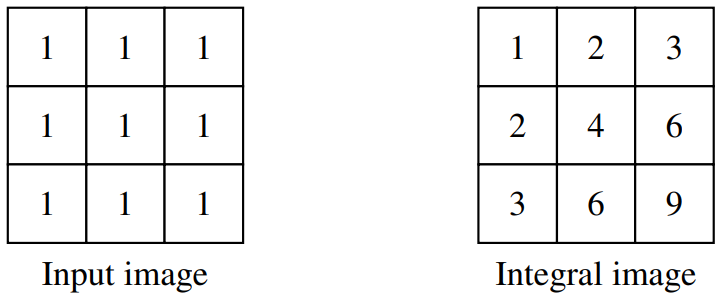
\includegraphics[scale=.3]{figs/imagem-integral.png}
    \legend{Fonte: Wikipedia (2020)}
    \label{fig:integral}
\end{figure}

Na Figura \ref{fig:integral} é demonstrado um exemplo onde os valores dos pixels da imagem original estão a esquerda e os valores da imagem integral resultante estão a direita.

O cálculo é feito definindo o retângulo a ser analisado e então aplicando a Equação \eqref{eq:img-integral}. Tal equação é utilizada em \eqref{eq:img-integral-exemplo} para calcular soma dos valores do retângulo rosa da Figura \ref{fig:integral} que inclui os pontos 15, 16, 14, 28, 27 e 11. A correspondência das cores demarcadas na figura \ref{fig:integral} com as variáveis da Equação \eqref{eq:img-integral} se da por A - amarelo, B - verde, C - azul e D - rosa.

\begin{align}\label{eq:img-integral}
    \text{ Soma dos valores do retângulo } & = D - (B + C) + A               \\
    \label{eq:img-integral-exemplo}
    15 + 16 + 14 + 28 + 27 + 11            & = 101 - (254 + 186) + 450 = 111
\end{align}

Com a possibilidade de calcular facilmente a soma dos pixels de um retângulo arbitrário de forma rápida, o algoritmo para detecção pode analisar diversos trechos da imagem, chamados aqui de características, fazendo a comparação de duas ou mais áreas retangulares predefinidas, como os exemplos ilustrado na Figura \ref{fig:features}, onde as áreas demarcadas em cinza e branco compõe juntas uma única característica. O valor final de cada característica é definido pela soma do valor dos pixels sob o retângulo cinza menos a soma do valor dos pixels sob o retângulo branco.

\begin{figure}[htb]
    \centering
    \caption{Exemplos de características retangulares analisadas.}
    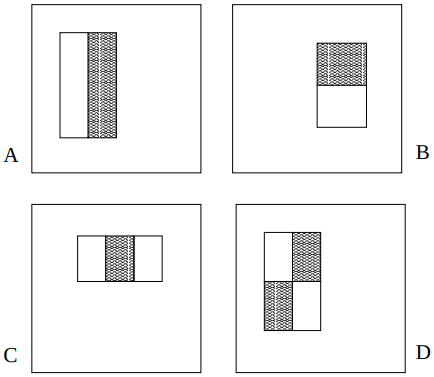
\includegraphics[scale=.5]{figs/features.png}
    \legend{Fonte: \citeauthoronline{paper-viola-jones} (\citeyear{paper-viola-jones})}
    \label{fig:features}
\end{figure}

%-
\subsection{Algoritmo de AdaBoost e Classificador em Cascata}
%-

As características demonstradas anteriormente, são definidas basicamente como duas ou mais áreas retangulares de qualquer tamanho, tal simplicidade implica na possibilidade da criação de uma enorme variação das mesmas que precisam ser calculadas diversas vezes, para cada parte de imagem e com diferentes tamanhos, isso implica em um alto custo de processamento. Para evitar tal problema é utilizado o algoritmo de \textit{AdaBoost} \cite{adaboost-Freund}, que possibilita grande otimização na demanda de processamento do detector facial e consequente redução do tempo de execução.

No caso do algoritmo de detecção facial Viola-Jones, o algoritmo AdaBoost é utilizado em dois momentos principais, o primeiro deles ocorre na seleção do conjunto de características mais eficientes durante o treino para criação do arranjo ponderado de vários classificadores fracos que combinados adequadamente se tornam um classificador forte \cite{fabio-luciana-2015}. A Figura \ref{fig:top-features} retrata as melhores características registradas por \citeauthoronline{paper-viola-jones} \cite{paper-viola-jones}. Fica claro que as mesmas se destacam por evidenciar as regiões dos olhos e do nariz.

\begin{figure}[htb]
    \centering
    \caption{Características retangulares mais eficientes para detecção facial.}
    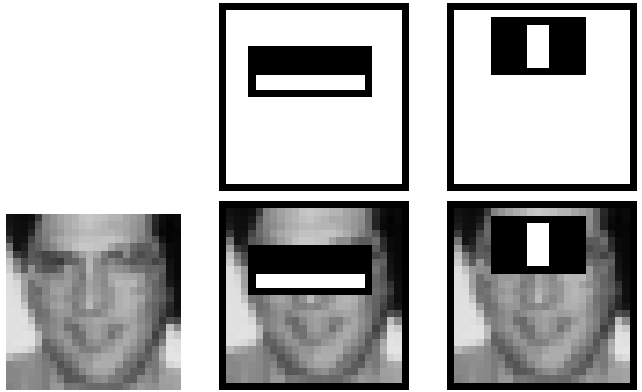
\includegraphics[scale=.4]{figs/top-features.png}
    \legend{Fonte: \citeauthoronline{paper-viola-jones} (\citeyear{paper-viola-jones})}
    \label{fig:top-features}
\end{figure}

É importante salientar que geralmente uma face não ocupa a maior parte de uma imagem a ser identificada, portanto é necessário encontrar uma forma rápida de descartar os elementos do fundo da mesma e concentrar o poder de processamento nos elementos que têm maior probabilidade de serem reconhecidos como uma face, isso leva a uma formulação para o problema onde ao contrário de encontrar faces, é necessário um algoritmo que descarte as ``não faces''.

Neste segundo momento, o AdaBoost apresenta uma boa solução, esta consiste na utilização do arranjo de classificadores já ponderados anteriormente, aplicados de forma sequencial, iniciando do mais fraco para o mais forte, criando o que é chamado de classificador em cascata, conforme ilustrado na Figura \ref{fig:cascade-classifier}, permitindo que imagens que certamente não possuem faces sejam rapidamente descartadas logo nas primeiras iterações, enquanto imagens com possíveis faces são classificadas por toda cascata, trazendo um elevado nível de confiança ao resultado.

\begin{figure}[htb]
    \centering
    \caption{Diagrama do funcionamento do classificador em cascata.}
    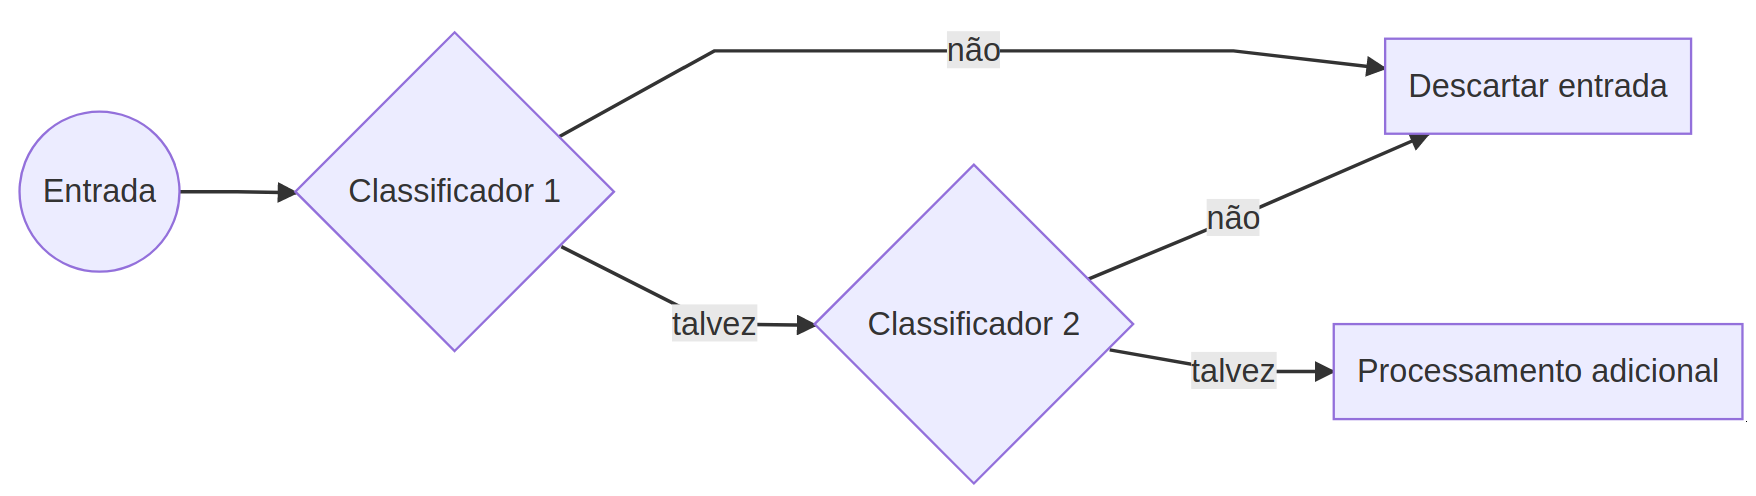
\includegraphics[scale=.2]{figs/cascade-classifier.png}
    \legend{Fonte: Própria (2020)}
    \label{fig:cascade-classifier}
\end{figure}

Um classificador comum, com um único estágio normalmente aceitaria muitos casos de falso negativo, para reduzir a taxa de falsos positivos e de descarte de imagens relevantes, mas no classificador em cascata, falsos positivos nos primeiros estágios não são um problema, pois serão analisados em outros diversos estágios e provavelmente eliminados.

A utilização desse modelo combinada com o algoritmo \textit{AdaBoost}, possibilita a análise das característica mais eficientes logo no início e consequentemente o descarte muito mais rápido dos casos negativos nos primeiros estágios.

%-
\subsection{OpenCV}
%-

A ferramenta \textit{OpenCV} foi utilizada neste trabalho para a implementação do método de Viola-Jones. Ela pode ser encontrada no website Github \footnote{OpenCV: https://github.com/itseez/opencv}, é uma biblioteca de código aberto focada na solução de problemas utilizando visão computacional em tempo real, desenvolvida pela Intel e posteriormente pela Itseez, com suporte a múltiplas plataformas e uso gratuito sobre licença de código aberto. A ferramenta apresenta suporte a arcabouços de aprendizado profundo, como TensorFlow \footnote{TensorFlow: https://www.tensorflow.org}, Pytorch \footnote{PyTorch: https://pytorch.org} e Caffe \footnote{Caffe: http://caffe.berkeleyvision.org} e contempla tanto funções básicas, para aplicações como processamento de imagem, alteração de cor ou resolução, até aplicações avançadas, como detecção facial, identificação de características e biometria \cite{wiki:OpenCV}.

A detecção de faces utilizando OpenCV consiste em duas etapas principais: a primeira consiste no treinamento do modelo, onde são apresentadas diversas imagens já identificadas para que o modelo encontre padrões positivos e negativos. Após o treinamento, a segunda etapa consiste em utilizar o modelo obtido para identificar, em novas imagens, características semelhantes as vistas nas imagens do treinamento. Neste projeto, será utilizado um modelo fornecido em conjunto com a ferramenta OpenCV, já treinado com diversos exemplos de faces frontais.

%-
\subsection{Parametrização do Algoritmo}\label{sec:parametrizacao}
%-

O procedimento de detecção facial utilizando o OpenCV permite ainda o ajuste de parâmetros para a execução do algoritmo de Viola-Jones.

O primeiro deles é chamado \textit{fator de escala}, que é o fator pelo qual as dimensões da janela de análise serão multiplicadas na tentativa de encontrar faces de diferentes tamanhos, pois o modelo é preparado para reconhecer faces de um tamanho específico, então durante a detecção a imagem é redimensionada e reanalisada diversas vezes para que faces de diferentes tamanhos possam ser detectadas. Para ajuste deste parâmetro, deve-se considerar que quanto mais próximo de 1 o seu valor, maior a chance de encontrar faces, mas a execução do detector também se torna mais custosa em termos de processamento.

O segundo parâmetro é o \textit{número mínimo de vizinhos}, que especifica quantos vizinhos cada retângulo candidato deve ter para retê-lo. Em mais detalhes, o detector analisa imagens utilizando um método de janelas retangulares que selecionam a partes da imagem, cada parte tem seus padrões comparados com os padrões de uma face e então é definido se esta janela contém ou não uma face, mas devido as várias iterações do detector sobre a mesma imagem durante a análise, pode ocorrer a sobreposição de janelas detectadas e então uma mesma face pode ser detectada em mais de uma janela, tais janelas são consideradas janelas vizinhas, pois foram duas detecções que ocorreram em diferentes varreduras mas estão sobre uma mesma área da imagem.

Portanto para melhorar a precisão do detector e também filtrar detecções duplicadas, o parâmetro de número mínimo de vizinhos define quantas janelas vizinhas devem existir para considerar aquela parte da imagem como uma face. Enfim, para ajuste deste parâmetro, deve-se considerar que, quanto mais próximo de zero o seu valor, maior a chance de detectar faces, mas, consequentemente, maior a chance de falsos positivos.

Por exemplo, caso o parâmetro de número mínimo de vizinhos seja igual a zero, qualquer janela que detectar uma face, em qualquer uma das varreduras, será considerada como uma face no resultado final. Já com o parâmetro igual a 4, é necessário que a mesma região da imagem seja considerada face por 4 janelas de varreduras diferentes para ser considerada como uma única face no resultado final. Esse comportamento pode ser observado nos resultados apresentados na Figura \ref{fig:min-neighbors-messi}.

\begin{figure}[htb]
    \centering
    \caption{Resultados da detecção com variação de parâmetros.}
    \legend{Utilizando o parâmetro de número mínimo de vizinhos igual a 0 (esquerda), 2 (centro) e 4 (direita).}
    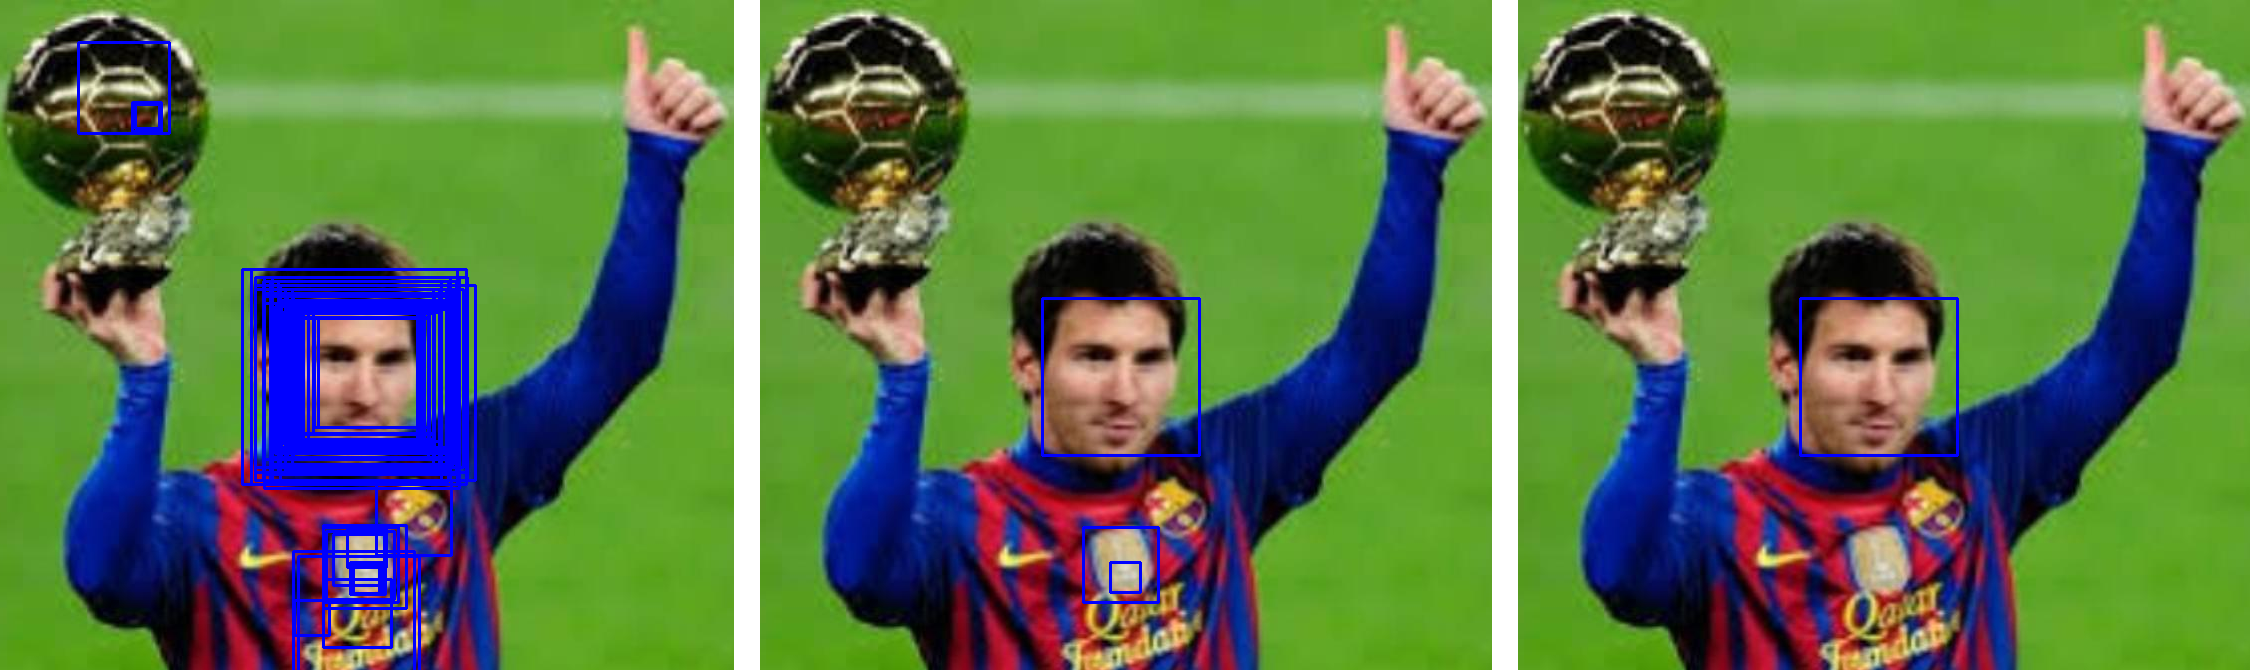
\includegraphics[scale=.2]{figs/min_neighbors_messi.png}
    \legend{Fonte: Própria (2020)}
    \label{fig:min-neighbors-messi}
\end{figure}

\section{Rede Neural Convolucional}

Uma das ferramentas que tem ganhado maior destaque na área de visão computacional recentemente são as redes neurais profundas, principalmente os algoritmos de redes neurais convolucionais, devido à sua poderosa capacidade de detectar padrões mais complexos \cite{gu2018recent}. Uma \textit{rede neural convolucional} (CNN, \textit{convolutional neural network}) funciona aplicando filtros com variados pesos às imagens de entrada, possibilitando assim a detecção de padrões específicos. A principal diferença em relação ao método de Viola-Jones é que aqui os filtros e seus pesos são inicialmente aleatórios e, então, automaticamente ajustados durante o treinamento da rede.

Os filtros, aplicados através da operação de convolução, permitem detectar padrões simples, como linhas e curvas; mas, com o treinamento e a combinação de uma grande quantidade de filtros, é possível detectar características de maior complexidade, como objetos, animais ou faces. Além disso, a operação de convolução ainda pode ser aplicada de forma que o tamanho da imagem resultante seja menor que o tamanho da imagem de entrada, mas mantendo as características mais importantes, o que faz com que a necessidade de poder computacional para o restante da análise seja reduzida \cite{cnn_face_detection}.

Além da etapa de convolução com filtros, outras duas etapas igualmente importantes são aplicadas às imagens na rede neural. A primeira delas é a aplicação de uma função de ativação, que costuma ser não linear, como a função de \textit{Unidades lineares retificadas} (ReLU, \textit{Rectified Linear Units}), que transforma todos valores resultantes negativos em zero sem alterar os valores positivos \cite{relu_ide2017improvement}. A segunda etapa aplicada sobre a imagem é a de agrupamento, que tem a função de reduzir o tamanho da imagem, com o objetivo de agilizar o treinamento e obter invariância ao deslocamento das features, tal redução é feita agrupando pixels próximos utilizando funções como o valor máximo ou médio entre os pixels da entrada \cite{vargas2016estudo}.

\subsection{TensorFlow e Keras}

Para este trabalho foram utilizadas três ferramentas que facilitam a aplicação da CNN. A primeira delas é chamada TensorFlow, uma plataforma de código aberto que disponibiliza ferramentas de aprendizado de máquina. A segunda ferramenta, Keras, disponibiliza uma interface em linguagem python para utilização de plataformas como TensorFlow, facilitando bastante a utilização da mesma para o usuário final.

Adentrando a área de detecção facial especificamente, um método popular é o de MTCNN, pois consegue atingir resultados bons não apenas para detecção de faces completas, mas também de partes da face, como olhos e boca. \cite{mtcnn}

\subsection{MTCNN}

No método MTCNN, a estrutura em cascata consiste em três redes, no pré-processamento a imagem é redimensionada para uma variedade de tamanhos diferentes (chamada de pirâmide de imagens), depois a primeira rede (Rede de propostas) propõe regiões candidatas a conterem faces, então a segunda rede (Rede de refinamento) filtra as regiões específicas que delimitam as posições das faces detectadas; e, por fim, a terceira rede (Rede de saída) propõe pontos de referência faciais como olhos e boca. Este método se assemelha bastante ao classificador em cascata do método de Viola-Jones, onde são utilizadas ferramentas mais simples para um filtragem inicial, e então a complexidade das análises aumenta nas regiões onde possivelmente pode ser encontrada uma face \cite{mtcnn}. Os resultados de cada uma das etapas podem ser visualizados na Figura \ref{fig:mtcnn}.

\begin{figure}[htb]
    \centering
    \caption{Resultados de cada etapa do método MTCNN.}
    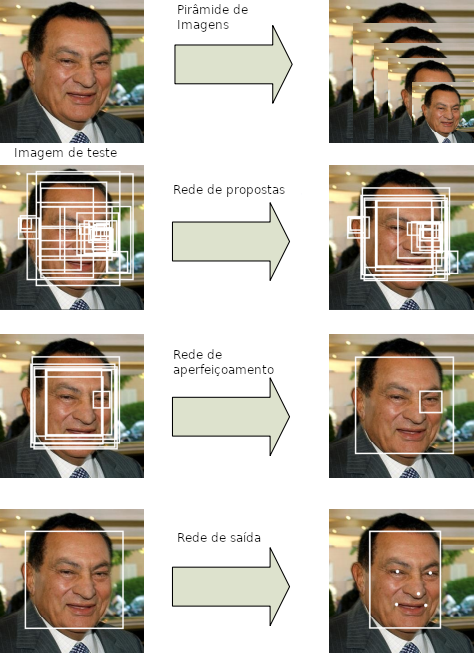
\includegraphics[scale=.8]{figs/mtcnn.png}
    \legend{Fonte: \citeauthoronline{mtcnn} \citeyear{mtcnn}}
    \label{fig:mtcnn}
\end{figure}

Neste trabalho, foi utilizada uma implementação do método MTCNN que utiliza Python, TensorFlow e Keras, e está disponível no github \cite{mtcnn_github}. Esta implementação possui um modelo já treinado que, a partir de uma imagem de entrada, fornece a posição das faces detectadas, assim como a confiança de que a mesma é realmente uma face e a posição dos pontos de referência (olhos, nariz e boca). Para análise, todas as faces detectadas foram consideradas, independente da confiança na detecção, pois assim os resultados melhor satisfazem a necessidade deste projeto.

\section{Conjuntos de imagens para teste}

Para analisar a eficiência da implementação do algoritmo \textit{Viola-Jones} na biblioteca \textit{OpenCV}, assim como o seu modelo previamente treinado, foram selecionadas manualmente 500 imagens retiradas de dois conjuntos de imagens disponíveis na internet.

\subsection{Conjuntos de imagens originais}

O primeiro conjunto de imagens, nomeado UTKFace \cite{utkface}, consiste em um conjunto de mais de 20 mil imagens, com uma única face em cada, de diversas pessoas entre 0 e 116 anos de idade, catalogadas de acordo com idade, raça e sexo. Alguns exemplos das imagens contidas no dataset podem ser vistos na Figura \ref{fig:exemplos-utk}.

\begin{figure}[htb]
    \centering
    \caption{Exemplos de imagens do dataset UTKFace.}
    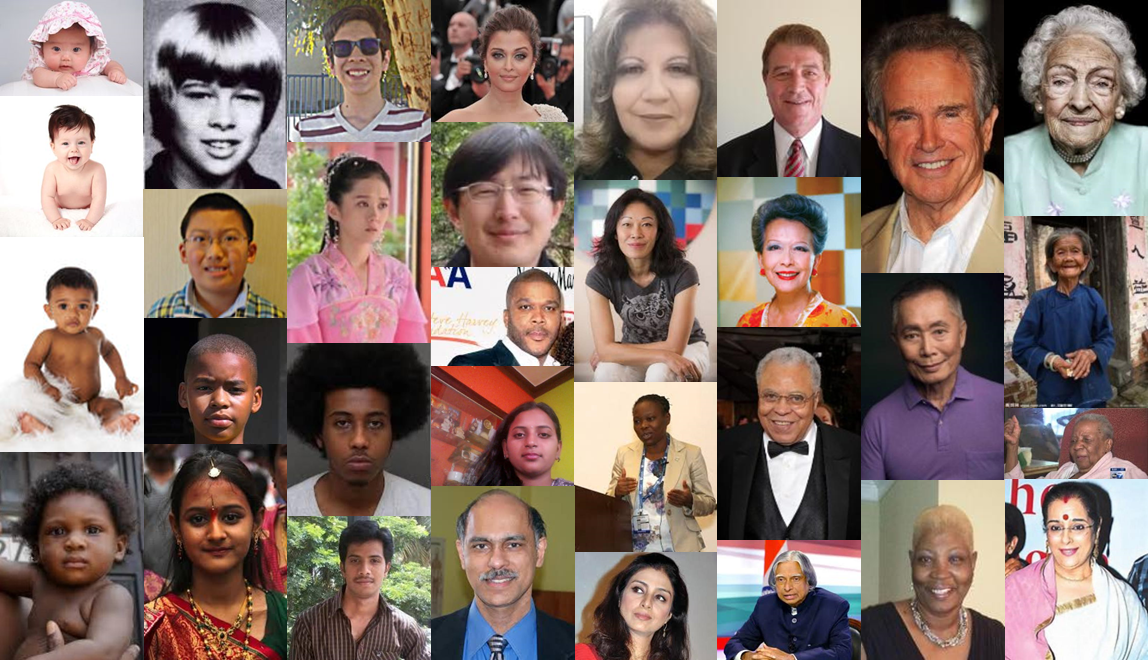
\includegraphics[scale=.3]{figs/exemplos-utk.png}
    \legend{Fonte: UTKFace dataset \cite{utkface}}
    \label{fig:exemplos-utk}
\end{figure}

O segundo conjunto de imagens, nomeado \textit{Hotels-50k} \cite{hotels50k-article}, consistia originalmente em mais de 50 mil fotografias de diversos quartos de hotel vazios. Este foi utilizado pois imagens com características semelhantes a estas são muitas vezes submetidas erroneamente em cadastros pessoais, em vez de uma imagem da face a ser cadastrada.

\subsection{Conjunto de imagens selecionadas}

Para os testes, foi selecionado manualmente um conjunto com 400 imagens positivas (possuíam uma face válida) e 100 imagens negativas (não possuíam uma face válida). Tal proporção representa a hipótese de que cerca de 20\% de imagens enviadas para cadastros, na verdade, não possuem uma face.

Por considerar que as imagens avaliadas pelo detector facial estudado neste trabalho serão utilizadas para cadastros pessoais e, portanto, é necessário que demonstrem que houve o consentimento de quem estava sendo fotografado e que seja possível identificar com clareza a pessoa da foto, as 400 imagens positivas (exemplos na Figura \ref{fig:valid-faces}) foram selecionadas manualmente de forma que cumprissem os critérios abaixo.

\begin{itemize}
    \item A imagem deve conter uma única face frontal;
    \item Olhos, nariz e boca devem estar visíveis;
    \item A pessoa fotografada deve ter entre 18 e 60 anos;
    \item A pessoa fotografada deve estar olhando para a câmera;
    \item A imagem deve ter boa definição e foco;
    \item A face deve estar centralizada e próxima da câmera.
\end{itemize}

\begin{figure}[htb]
    \centering
    \caption{Exemplos de imagens com face válida.}
    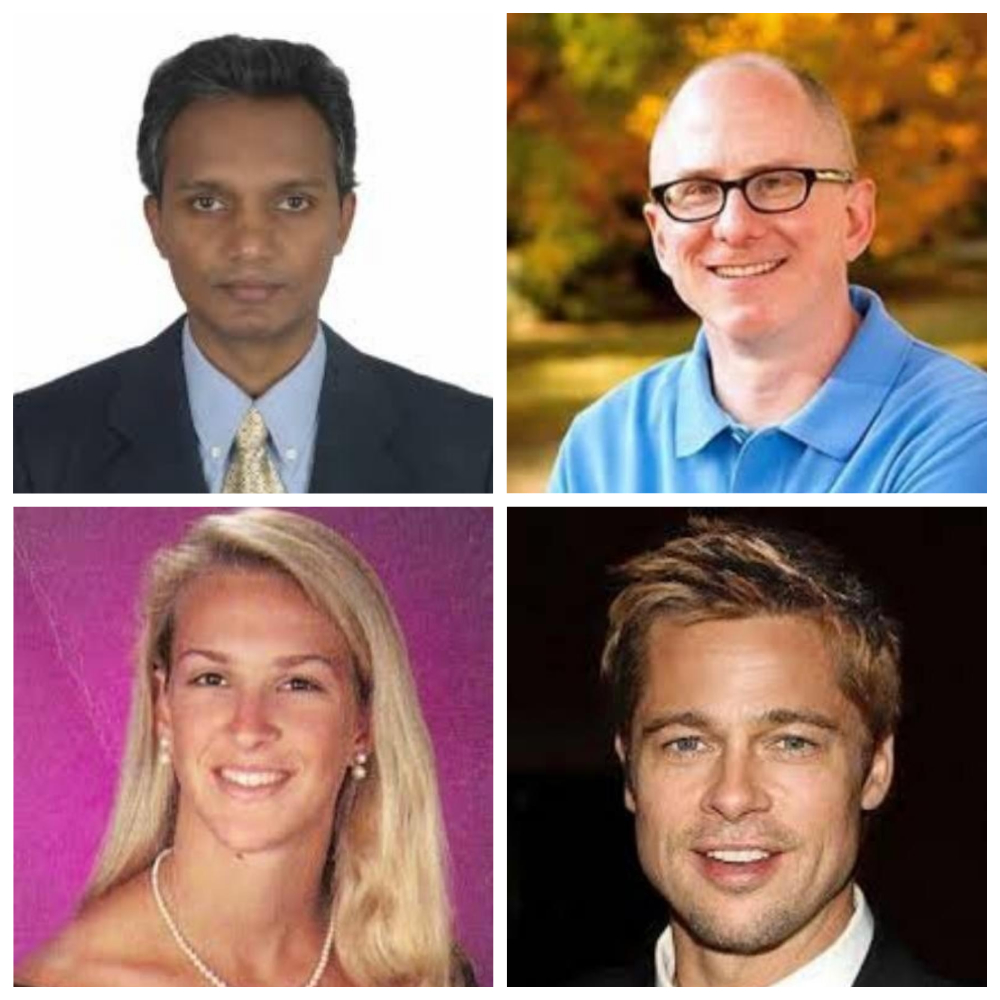
\includegraphics[scale=.25]{figs/valid_faces.jpg}
    \legend{Fonte: \textit{UTKFace dataset} \cite{utkface}}
    \label{fig:valid-faces}
\end{figure}

É preciso considerar também que existem imagens que contém faces, mas que não são válidas, pois não cumprem os critérios definidos, portanto essas devem ser consideradas negativas. Para maior confiabilidade nos testes feitos, o grupo de imagens negativas foi composto por 30 imagens que apresentavam faces inválidas (exemplos na Figura \ref{fig:invalid-faces}) e outras 70 imagens selecionadas aleatoriamente do conjunto \textit{Hotels-50k} (exemplos na Figura \ref{fig:hotel-examples}).

\begin{figure}[tbp]
    \centering
    \caption{Exemplos de imagens com face inválida.}
    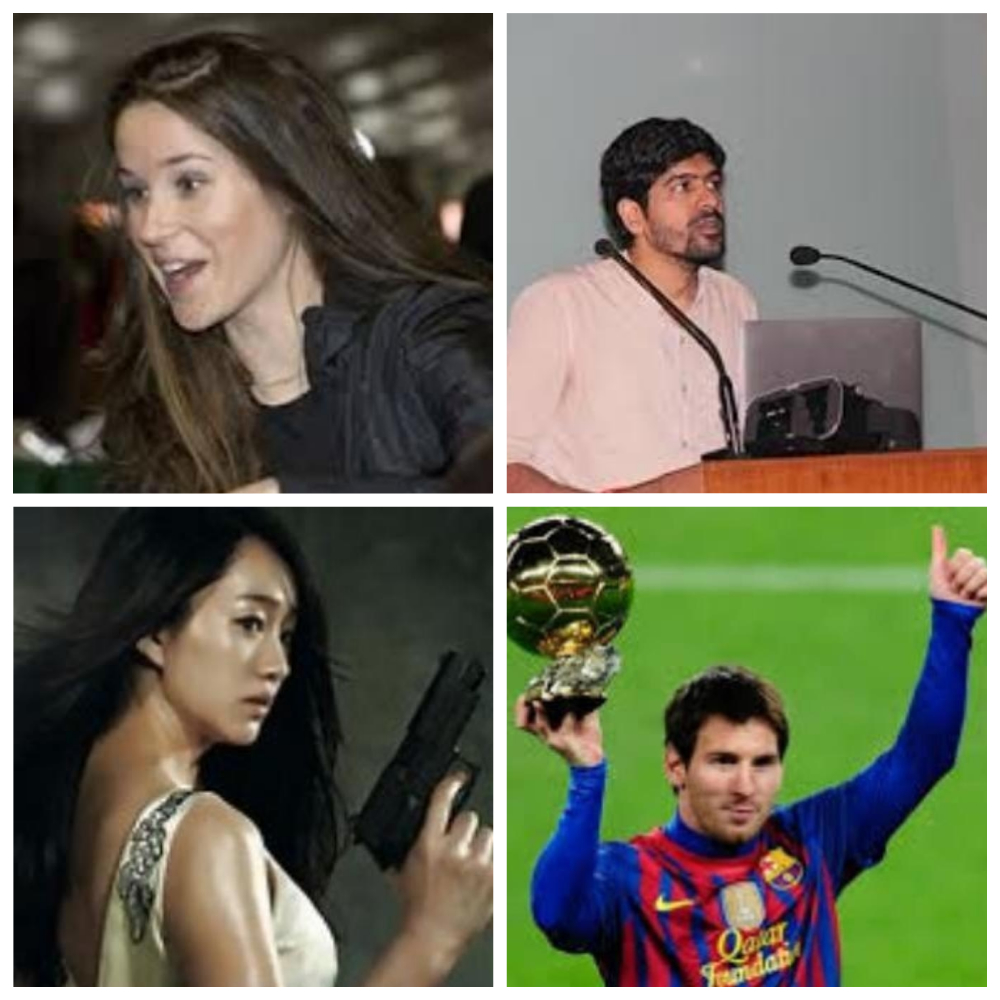
\includegraphics[scale=.25]{figs/invalid_faces.jpg}
    \legend{Fonte: \textit{UTKFace dataset} \cite{utkface}}
    \label{fig:invalid-faces}
\end{figure}

\begin{figure}[tbp]
    \centering
    \caption{Exemplos de imagens sem nenhuma face.}
    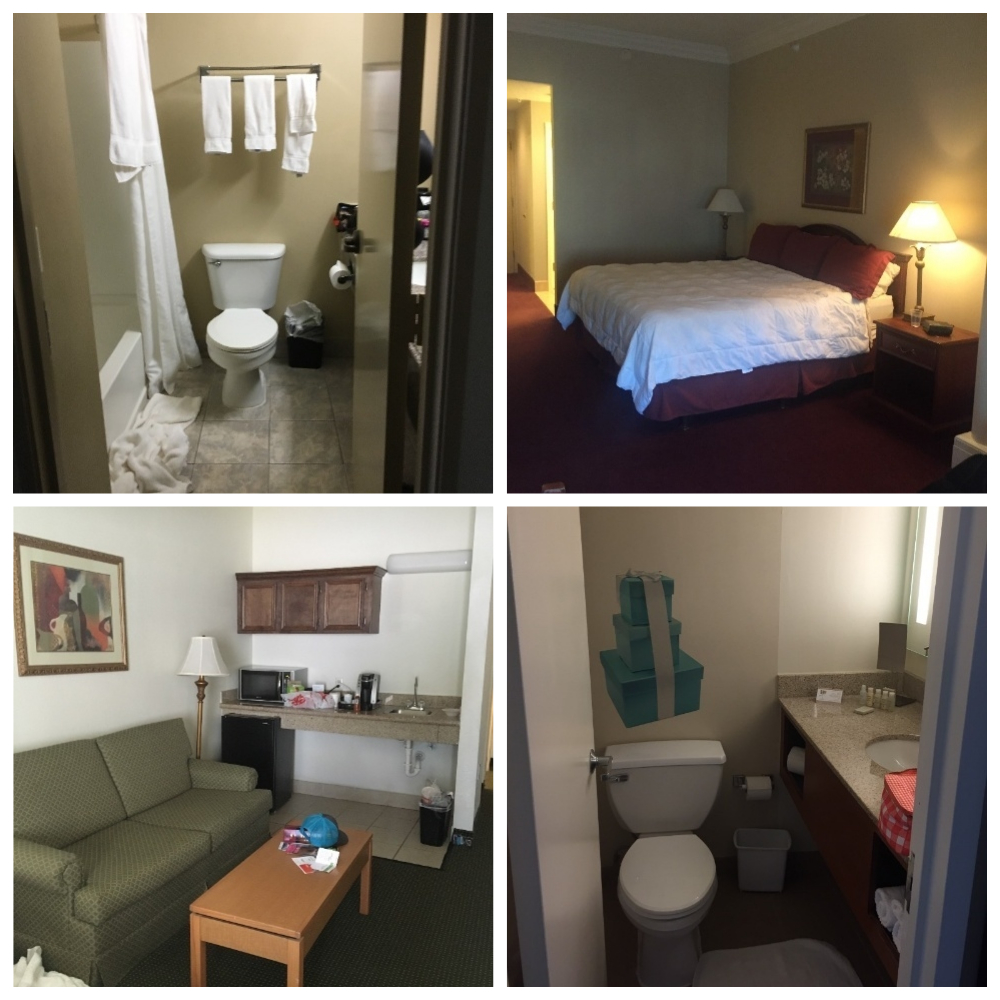
\includegraphics[scale=.25]{figs/hotels.jpg}
    \legend{Fonte: \textit{Hotels-50k dataset} \cite{hotels50k-article}}
    \label{fig:hotel-examples}
\end{figure}

%-
\section{Metodologia de Análise}
%-

Para melhor analisar os resultados dos testes, foi necessário especificar com clareza como poderiam ser agrupadas as imagens, dada a sua origem e o resultado observado no teste. Para isso foram utilizadas as definições da Tabela \ref{tab:conjuntos-images}.

\begin{table}[htbp]
    \caption{Conjuntos observados.}
    \label{tab:conjuntos-images}
    \centering
    \renewcommand{\arraystretch}{1.4}
    \begin{tabular}{ccc}\hline\hline
        \textbf{Conjunto} & \textbf{Descrição}                                     & \textbf{Quantidade} \\
        \midrule
        \textit{A}        & Imagens que contêm uma face válida                     & 400                 \\
        $\overline{A}$    & Imagens que não contêm uma face válida                 & 100                 \\
        \textit{B}        & Imagens onde o algoritmo identificou uma ou mais faces & Variável            \\
        $\overline{B}$    & Imagens onde o algoritmo não identificou nenhuma face  & Variável            \\
        \hline\hline
    \end{tabular}
\end{table}

Definidos os conjuntos, pode-se utilizar a matriz de confusão da Tabela \ref{tab:matriz_de_confusao} para facilitar a análise da relação entre os conjuntos definidos anteriormente. Na Tabela \ref{tab:matriz_de_confusao} são observados os conjuntos \textit{a - verdadeiro positivo} (TP, \textit{true positive}) em que o algoritmo identifica corretamente uma face em cada uma das imagens que realmente contém uma face, \textit{b - falso negativo} (FN, \textit{false negative}) em que o algoritmo erroneamente não reconheceu nenhuma face, apesar das imagens conterem uma face cada, \textit{c - falso positivo} (FP, \textit{false positive}) em que o algoritmo erroneamente identificou ao menos uma face, mesmo as imagens não contendo nenhuma e \textit{d - verdadeiro negativo} (TN, \textit{true negative}) em que o algoritmo identificou corretamente que não existia nenhuma face nas imagens. É importante destacar que os quatro conjuntos destacados na matriz de confusão são mutuamente excludentes \cite{Dougherty:2012:PRC:2553126}.

\begin{table}[htbp]
    \caption{Matriz de confusão.}
    \label{tab:matriz_de_confusao}
    \centering
    \renewcommand{\arraystretch}{1.4}
    \begin{tabular}{c|cc}
        \hline\hline
                       & \textit{B}                       & $\overline{B}$                   \\
        \hline
        \textit{A}     & \textit{a} (verdadeiro positivo) & \textit{b} (falso negativo)      \\
        $\overline{A}$ & \textit{c} (falso positivo)      & \textit{d} (verdadeiro negativo) \\
        \hline\hline
    \end{tabular}
\end{table}

Para melhor entender os agrupamentos da matriz de confusão, pode-se observar na Figura \ref{fig:norm_dist} as distribuições que representam a quantidade de imagens dos conjuntos \textit{A} e $\overline{A}$ dada a sua probabilidade de conter uma face. Nesse exemplo deve-se supor o uso de apenas uma caracterísca, mostrada de modo ilustrativo.

\begin{figure}[htb]
    \centering
    \caption{Exemplo teórico de uma distribuição normal dos grupos de uma matriz de confusão.}
    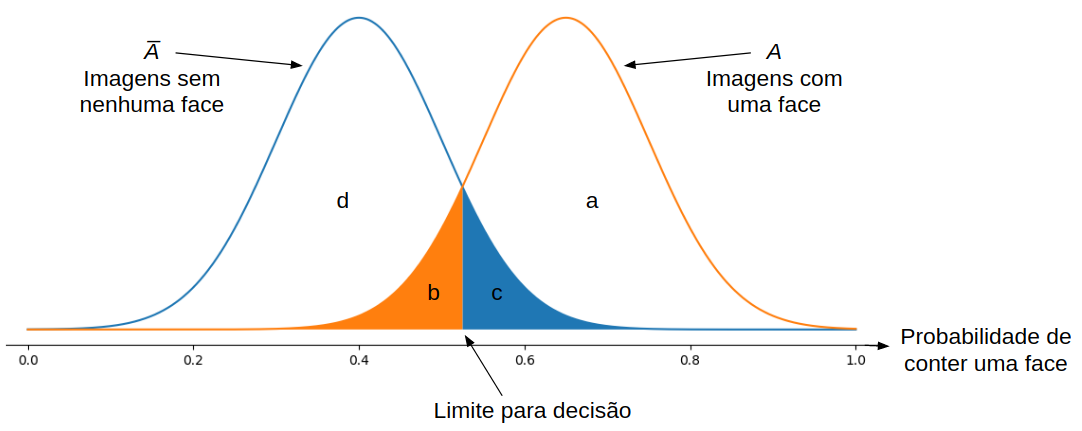
\includegraphics[scale=.4]{figs/norm_dist.png}
    \legend{Fonte: Própria (2020)}
    \label{fig:norm_dist}
\end{figure}

Nas distribuições são destacados os grupos \textit{b} (falso negativo) e \textit{c} (falso positivo) e fica evidente que, devido à sobreposição das distribuições \textit{A} e $\overline{A}$, é necessário definir um limite para decisão, que pode ser ajustado conforme a necessidade, mas, que independente do seu ajuste, sempre existirá um grupo categorizado de forma incorreta.

A matriz de confusão também pode ser escrita em termos probabilísticos (Tabela \ref{tab:matriz_de_confusao_probab}), incluindo as probabilidades marginais, ou pode ser visualizada no diagrama de Venn correspondente (Figura \ref{fig:venn_diagram}).

\begin{table}[htbp]
    \caption{Matriz de confusão com probabilidades marginais.}
    \label{tab:matriz_de_confusao_probab}
    \centering
    \renewcommand{\arraystretch}{1.4}
    \begin{tabular}{c|cc|c}\hline\hline
                       & \textit{B}               & $\overline{B}$                      & Soma              \\
        \hline
        \textit{A}     & $P(A \cap B)$            & $P(A \cap \overline{B})$            & $P(A)$            \\
        $\overline{A}$ & $P(\overline{A} \cap B)$ & $P(\overline{A} \cap \overline{B})$ & $P(\overline{A})$ \\
        \hline
        Soma           & $P(B)$                   & $P(\overline{B})$                   & 1                 \\
        \hline\hline
    \end{tabular}
\end{table}

\begin{figure}[htb]
    \centering
    \caption{Diagrama de Venn para as imagens analisadas.}
    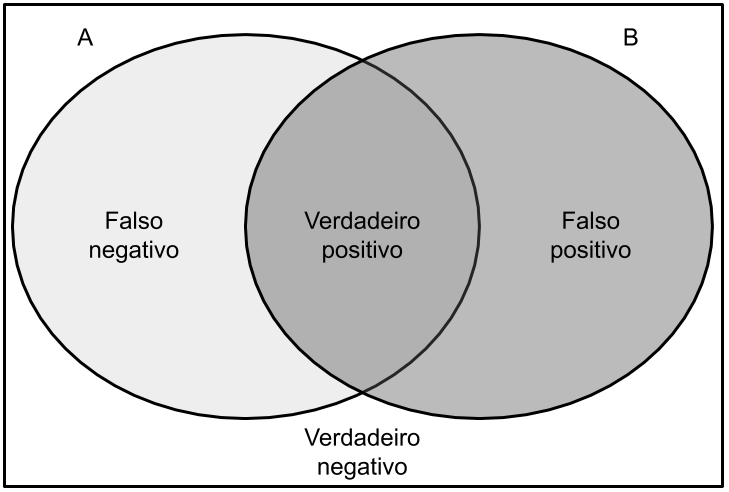
\includegraphics[scale=.4]{figs/venn-diagram.png}
    \legend{Fonte: Própria (2020)}
    \label{fig:venn_diagram}
\end{figure}

Podem também ser calculadas as medidas tradicionais de sensibilidade (a probabilidade condicional de o algoritmo identificar ao menos uma face dado que a imagem contém uma face) e especificidade (a probabilidade condicional de o algoritmo não identificar qualquer face em uma imagem que realmente não contenha faces) conforme as Equações \eqref{eq:sensibilidade} e \eqref{eq:especificidade}.

\begin{align} \label{eq:sensibilidade}
    \text{sensibilidade, } P(B|A) = P(A \cap B) / (P(A \cap B) + P(A \cap \overline{B})) = a/(a + b) \\
    \label{eq:especificidade}
    \text{especificidade, } P(\overline{B} | \overline{A}) = P(\overline{A} \cap \overline{B}) / (P(\overline{A} \cap \overline{B}) + P(\overline{A} \cap B)) = d/(d + c)
\end{align}

Por fim, a partir da sensibilidade e especificidade, é possível exibir o resultado do classificador no espaço de característica operacional do receptor (ROC, \textit{receiver operating characteristic}), que consiste em um plano em que o eixo horizontal mede a taxa de falsos positivos (1 - especificidade) e o eixo vertical mede a taxa de verdadeiros positivos (sensibilidade). Isso permite comparar facilmente diferentes classificadores, pois, quanto mais próximo ao canto esquerdo superior, melhor a classificação.

\begin{figure}[htb]
    \centering
    \caption{Espaço ROC.}
    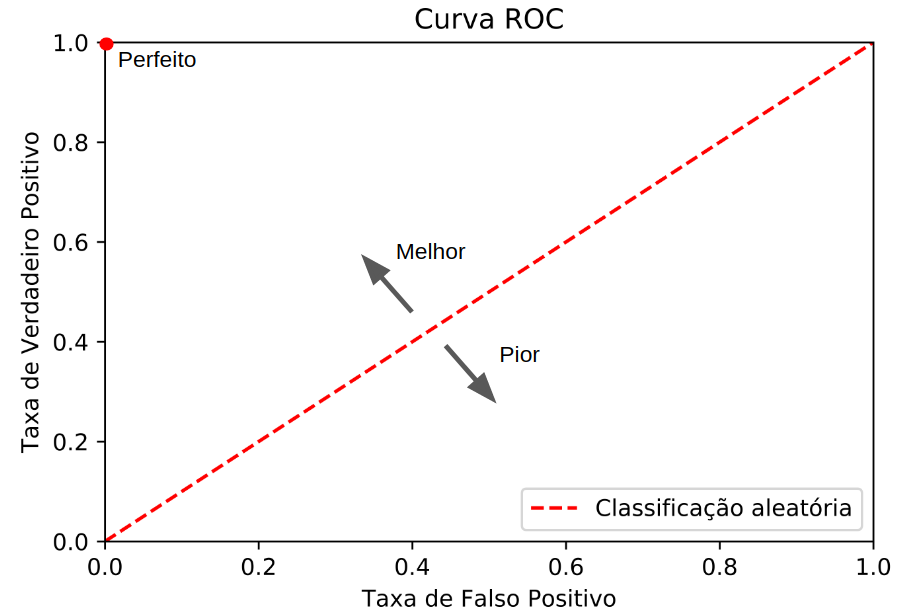
\includegraphics[scale=.4]{figs/curva_roc.png}
    \legend{Fonte: Própria (2020)}
    \label{fig:roc_space}
\end{figure}

\section{Análise de Custo}

Para entender o valor da utilização de um modelo de reconhecimento facial para filtragem de imagens inválidas, pode-se utilizar o exemplo de uma empresa de cartões de crédito que precisa analisar fotos de clientes antes de lhes fornecer um cartão. Considerando como R o valor presente líquido \cite{npv-article}, ou seja, a receita total que este cliente traz para empresa, e H como o custo de trabalho humano para a análise de uma imagem, podemos calcular a receita da empresa antes e depois da aplicação de um modelo de detecção facial. Para as análises feitas neste trabalho, foi utilizado o valor presente líquido de R\$250,00 e o custo de análise de R\$ 1,00 \cite{hussain2007valuationnpv}.

Antes da aplicação do modelo, todas as fotos enviadas deveriam ser analisadas por um humano, gerando o custo de análise manual H, e apenas as fotos que continham uma face trariam a receita R para empresa, relacionando isso aos valores encontrados na matriz de confusão do modelo, pode-se obter o \textit{ganho inicial} ($g_0$) na Equação \eqref{eq:g_0}. Nesta equação tem-se o $Evento\:A = (TP + FN)$, que representa os casos cujas respectivas fotos contêm uma face, multiplicado pela receita de cada cliente R, subtraídos do custo de análise H multiplicado pela quantidade total de fotos recebidas, que equivale a soma de todas as taxas da matriz de confusão.

\begin{align} \label{eq:g_0}
    g_0 = (TP+FN) \times R - (TP+FP+FN+TN) \times H
\end{align}

Após a aplicação do modelo, apenas as fotos que foram classificadas pelo modelo como faces serão analisadas por humanos, gerando custo de análise manual H e apenas as fotos classificadas pelo modelo como face e que realmente contenham uma face se tornarão clientes reais, trazendo receita R para a empresa, com isso, pode-se obter o \textit{ganho final} ($g_1$) na Equação \eqref{eq:g_1}.
\begin{align} \label{eq:g_1}
    g_1 = TP \times R - (TP+FP) \times H
\end{align}

Para avaliar a receita que o modelo traz para a empresa, pode-se calcular a diferença entre a receita antes e depois do modelo, obtendo a Equação \eqref{eq:profit}.
\begin{align} \label{eq:profit}
    g_1 - g_0 = (FN + TN) \times H - FN \times R
\end{align}

Considerando que, para o modelo trazer valor para a empresa, é necessário que a receita após sua aplicação seja maior que a receita antes da sua aplicação, obtendo a Equação \eqref{eq:profit2}.
\begin{align} \label{eq:profit2}
    g_1 - g_0 > 0 \\
    (FN + TN) \times H - FN \times R > 0
\end{align}

A equação obtida ainda pode ser reescrita em função da \textit{taxa de verdadeiros positivos} (TPR, \textit{true positive rate}), que define quantos resultados verdadeiros positivos ocorrem entre todas as amostras positivas disponíveis, e da taxa de falsos positivos (FPR, \textit{false positive rate}), que define quantos resultados falsos positivos ocorrem entre todas as amostras negativas disponíveis durante o teste. Com esses valores é possível traçar a equação sobre o espaço ROC e visualizar de forma simples quais classificadores satisfazem o critério necessário para obtenção de receita. Para isso são consideradas a quantidade de imagens positivas ($ P = 0.8 $) e negativas ($ N = 0.2 $) definidas anteriormente e as relações \eqref{eq:FN_TPR} e \eqref{eq:TN_FPR}, obtendo por fim a Equação \eqref{eq:profit_roc} que pode ser exibida no espaço ROC na Figura \ref{fig:profit_roc}.

\begin{align}
    \label{eq:FN_TPR}
    FN  & = P \times (1-TPR)                                                                     \\
    \label{eq:TN_FPR}
    TN  & = N \times (1-FPR)                                                                     \\
    \label{eq:profit_roc}
    TPR & = 1 + \left( \frac{N}{P \times \left( \frac{R}{H}-1 \right) } \times (FPR - 1) \right)
\end{align}

\begin{figure}[htb]
    \centering
    \caption{Limiar lucrativo exibido no espaço ROC.}
    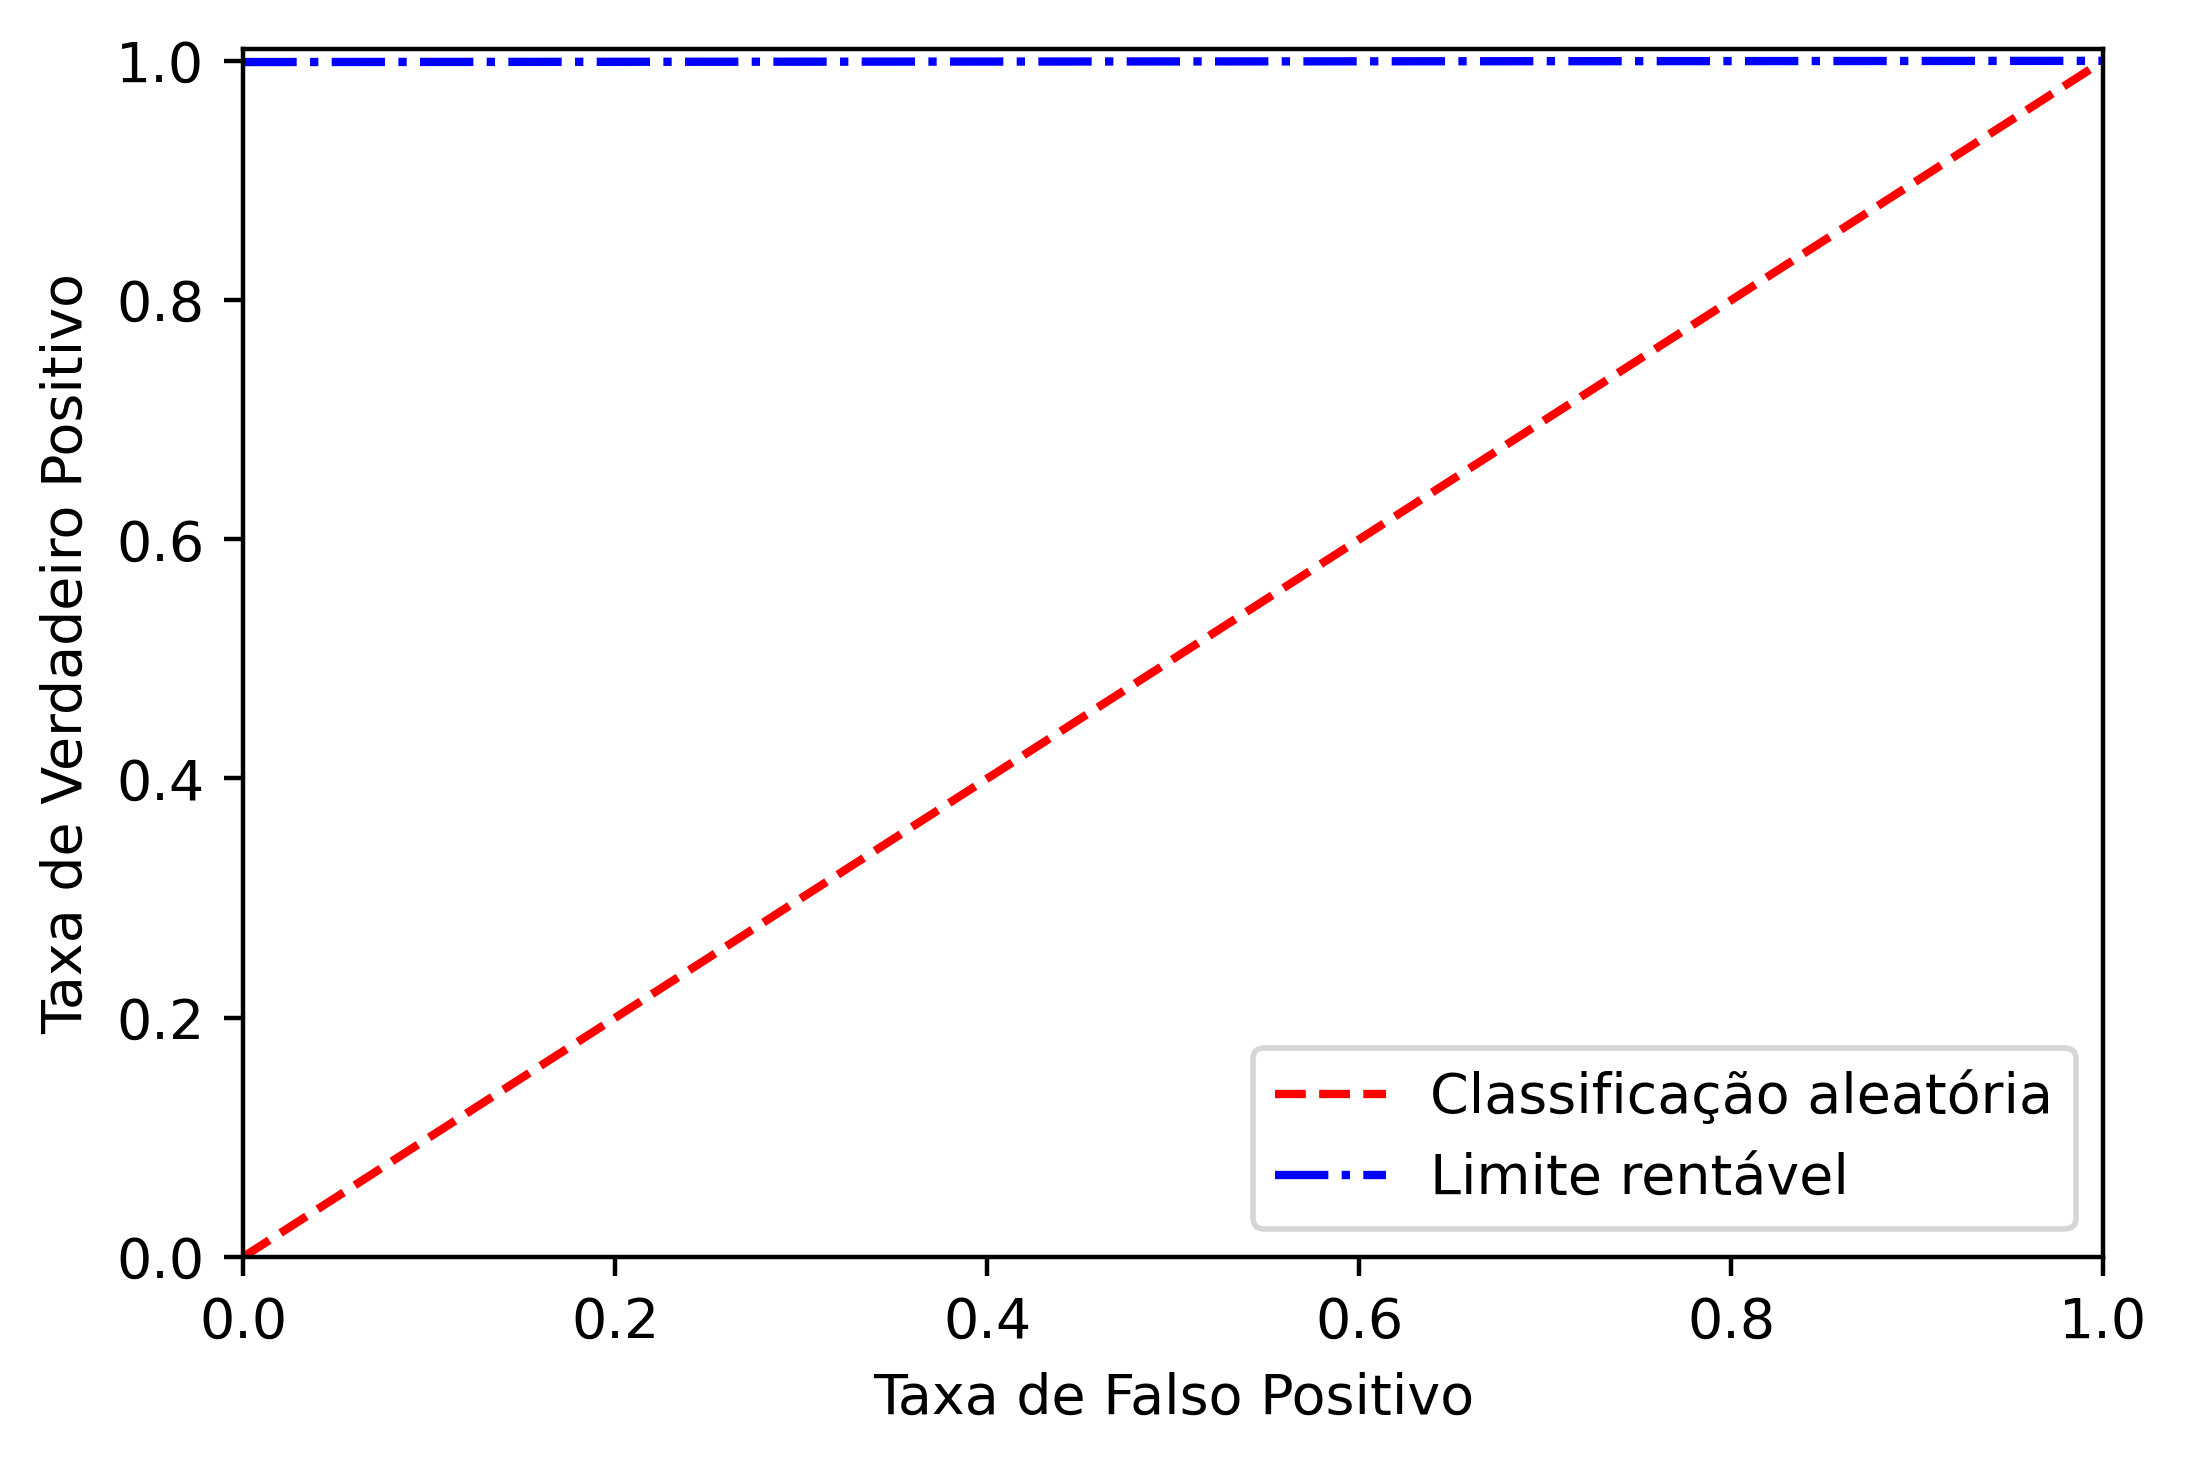
\includegraphics[scale=1]{figs/curva_roc_lucro.png}
    \legend{Fonte: Própria (2020)}
    \label{fig:profit_roc}
\end{figure}

Assim, é possível avaliar em função da matriz de confusão do modelo, do custo de análise manual de um documento, do valor presente líquido de um cliente e da proporção média de imagens positivas e negativas, se a aplicação deste modelo é viável ou não.
